\documentclass[10pt,aspectratio=169]{beamer}
\usepackage{poly}
\usepackage[backend=biber]{biblatex}
\addbibresource{bibliography.bib}
%\documentclass[10pt,aspectratio=169]{beamer}
\usepackage{poly}
\setbeamertemplate{caption}[numbered]

\usepackage[backend=biber]{biblatex}
\addbibresource{bibliography.bib}
\usepackage{eso-pic}

% ================================================================================
% Metadata
% ================================================================================
\title{
\vspace{1.5em}
Add you title here}
% \subtitle{Using \LaTeX\ to prepare slides}
\author{Group number: add group names here}
\institute[COMP]{Department of Engineering and Sciences
}
\date{\today}

% ================================================================================
% Main Body
% ================================================================================

\begin{document}
\maketitle % generate the title slide


\begin{frame}{\textbf{Title}}

Add a new slide by beginning a new frame. Here you can add what you want

\end{frame}



\begin{frame}{Research questions}
    \begin{enumerate}
        \item \textbf{Add your research questions here}
    \end{enumerate}
\end{frame}


\begin{frame}{Method}

\begin{columns}
    \begin{column}{0.5\textwidth}
        \begin{itemize}
            \item Explain your method here
\end{itemize}
    \end{column}

    \begin{column}{0.5\textwidth}
    \vspace{-1.8em}
    \begin{figure}
        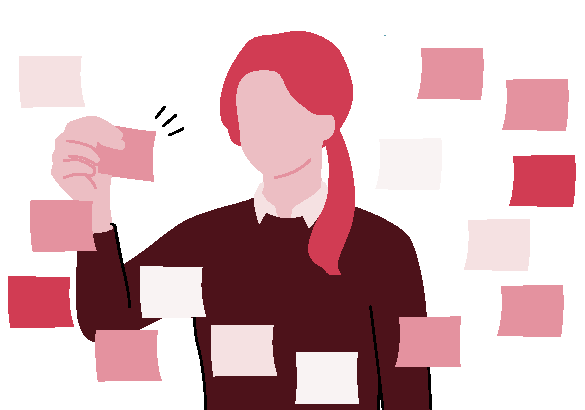
\includegraphics[width=0.95\linewidth]{source/post-it lapper.pdf}
        \vspace{-1em}
        \caption{UiA illustration from \cite{uia_illustrasjoner}}
    \end{figure}
\end{column}

\end{columns}

\end{frame}


\begin{frame}{Results}

Presents your results
    
\end{frame}


\begin{frame}{Discussion}

\begin{columns}
    \begin{column}{0.5\textwidth}
        \begin{itemize}
            \setlength{\itemsep}{1em}
            \item Discuss your method and results
        \end{itemize}
    \end{column}

    \begin{column}{0.5\textwidth}
    \vspace{-1.8em}
    \begin{figure}
        
\includegraphics[width=0.95\linewidth]{source/Attraktive studier.pdf}
        \vspace{-1em}
        \caption{UiA illustration from \cite{uia_illustrasjoner}}
    \end{figure}
\end{column}

\end{columns}


    
\end{frame}


\begin{frame}{Conclusion}

\textbf{Research questions:}
\begin{enumerate}
    \item Add your research question here
\end{enumerate}

\textbf{Main contributions include:}

\begin{enumerate}
    \item List your main contributions here
\end{enumerate}

\textbf{Future work}

\end{frame}

\begin{frame}[plain]
    \centering
    \vfill
    {\LARGE \textbf{Thank you for listening!}}
    \vfill
\end{frame}

\begin{frame}[allowframebreaks]{References}
    \printbibliography
\end{frame}



\end{document}